\section{Auswertung}
\label{sec:Auswertung}
Für die Temperatur wurde eine Messunsicherheit von $\symup{\Delta} T = 0.1$ angenommen.
\subsection{Statisches Vefahren}  
\subsubsection{Vergleich der Temperaturverläufe}
\begin{figure}
  \begin{subfigure}{0.48\textwidth}
    \centering
    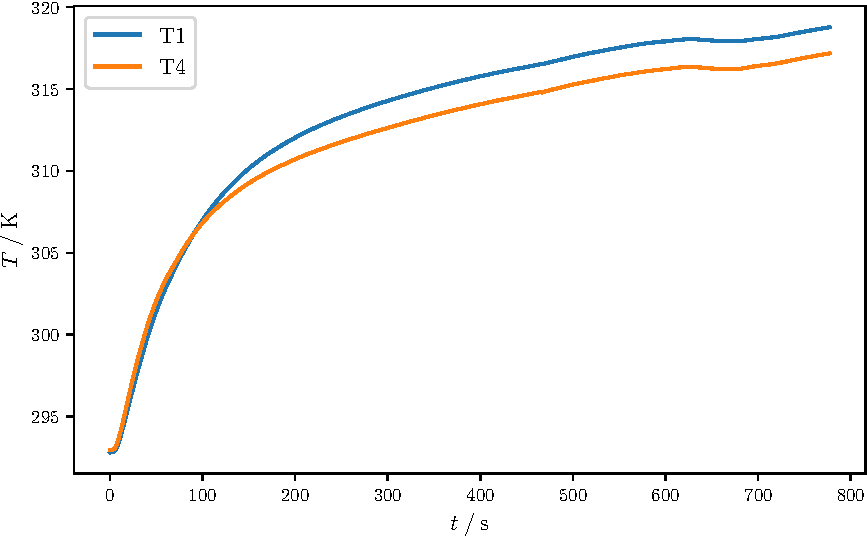
\includegraphics[width = \textwidth]{build/stat14.pdf}
    \caption{Temperaturverlauf $T_1$ und $T_4$}
    \label{fig:stat14}
  \end{subfigure}
  \begin{subfigure}{0.48\textwidth}
    \centering
    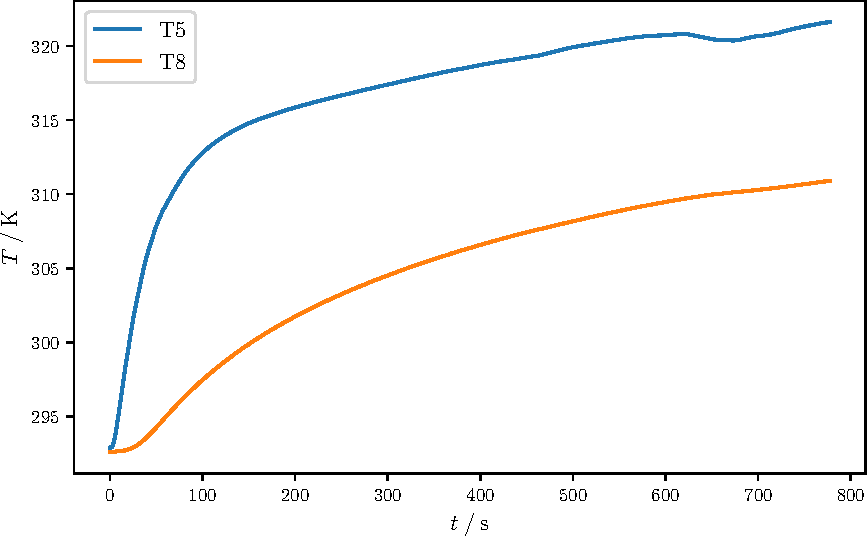
\includegraphics[width = \textwidth]{build/stat58.pdf}
    \caption{Temperaturverlauf $T_5$ und $T_8$}
    \label{fig:stat58}
  \end{subfigure}
\end{figure}
Bei dem Verglichen der Kurven fällt es auf, dass alle vier Kurven zu Beginn einen starken Temperaturanstieg repräsentieren, welcher jedoch schnell wieder abschwächt.
Dennoch verhalten sich die Temperaturen $T_1$ und $T_4$ Anfangs beinahe identisch, wobei die Temperaturen $T_5$ und $T_8$ dort Diskrepanzen aufzeigen. $T_5$ steigt 
sehr stark an und flacht vergleichsweise schnell wieder ab, während die Temperatur $T_8$ eine eher verhaltene Steigung aufweist, denn diese steigt sehr langsam an, besitzt
im Gegenzug daszu keinen abrupten Steigungsverlust. Nach dem beinahe identischen Verhalten, fällt die Kurve von $T_4$ früher ab, wonach dann eine kleine, annähernd konstante
Differenz zwischen den beiden Temperaturen herrscht. Aufgrund der verhaltenen Steigung der Temperaturkurve von $T_8$ ist die Differenz zwischen den beiden Kurven aus der 
Graphik \eqref{fig:stat58} schon von Anfang an sehr groß, wobei sich diese ab dem Zeitpunkt $t \approx \SI{150}{\second}$ eingestellt hat. Als letzte Gemeinsamkeit erkennt man leicht, dass
alle Kurven einen leichten Abfall bei $t \approx \SI{620}{\second}$ erleiden.
\subsubsection{Die beste Wärmeleitfähigkeit}
\begin{table}
  \centering
  \label{tab:Waeremleitfaehigkeit}
  \caption{Temperaturen nach $\SI{700}{\second}$}
  \sisetup{table-format = 3.2}
  \begin{tabular}{S S S S}
     \toprule
     {$T_1 \mathbin{/} \si{\kelvin}$} & {$T_4 \mathbin{/} \si{\kelvin}$} & {$T_5 \mathbin{/} \si{\kelvin}$} & {$T_8 \mathbin{/} \si{\kelvin}$}  \\
     \midrule
     318.06 & 316.42 & 320.66 & 310.28 \\
      \bottomrule
  \end{tabular}
\end{table}
Wie man anhand der Tabelle \eqref{tab:Waeremleitfaehigkeit} erkennen kann, hat Aluminium die beste Leitfähigkeit.
\subsubsection{Wärmestrom}
Für die Berechnung des Wärmestroms dient die Gleichung \eqref{eqn:Wärmemenge}. Jedoch lässt sich in diesem Fall die Wärmestromdichte
$j_w$ nicht mit dem Differntialquotient $\sfrac{\partial T}{\partial x}$ sondern nur mit dem Differenzenquotienten $\sfrac{\symup{\Delta}T}{\symup{\Delta} x}$
berechnen, so dass der Wärmestrom auch durch einen Differenzenquotienten dargestellt wird. 
Für den Abstand zwischen zwei Thermoelementen  wurde $\symup{\Delta} x = \SI{0.03}{\meter}$ gemessen.

\begin{table}
  \centering
  \caption{Errechnete Wärmeströme}
  \label{tab:Wärmestrom}
  \sisetup{table-format = 1.4}
  \begin{tabular}{S[table-format = 3.0] 
    S[table-format = 1.2] @{${}\pm{}$} S[table-format = 0.2] 
    S[table-format = 1.2] @{${}\pm{}$} S[table-format = 0.2] 
    S[table-format = 1.2] @{${}\pm{}$} S[table-format = 0.2] 
    S[table-format = 1.2] @{${}\pm{}$} S[table-format = 0.2]}
    \toprule
    {$t \mathbin{/} \si{\second}$} 
    & \multicolumn{2}{c}{$\frac{\symup{\Delta} Q_\text{Me}}    {\symup{\Delta}t} \mathbin{/} \si{\joule\second\tothe{-1}}$}
    & \multicolumn{2}{c}{$\frac{\symup{\Delta} Q_\text{Me,k}} {\symup{\Delta}t} \mathbin{/} \si{\joule\second\tothe{-1}}$}  
    & \multicolumn{2}{c}{$\frac{\symup{\Delta} Q_\text{Al}}    {\symup{\Delta}t} \mathbin{/} \si{\joule\second\tothe{-1}}$}
    & \multicolumn{2}{c}{$\frac{\symup{\Delta} Q_\text{St}}    {\symup{\Delta}t} \mathbin{/} \si{\joule\second\tothe{-1}}$}\\
    \cmidrule(lr){2-3} \cmidrule(lr){4-5} \cmidrule(lr){6-7} \cmidrule(lr){8-9}
    \midrule
    100 & 7.49 & 0.19 & 4.65 & 0.11 & 7.51 & 0.38 & 3.57 & 0.03 \\
    200 & 5.18 & 0.19 & 3.43 & 0.11 & 5.08 & 0.38 & 3.10 & 0.03 \\
    300 & 4.63 & 0.19 & 3.16 & 0.11 & 4.66 & 0.38 & 2.82 & 0.03 \\
    500 & 4.63 & 0.19 & 3.15 & 0.11 & 4.78 & 0.38 & 2.61 & 0.03 \\
    700 & 4.28 & 0.19 & 2.92 & 0.11 & 4.44 & 0.38 & 2.35 & 0.03 \\
    \bottomrule
  \end{tabular}
\end{table}
Der Fehler lässt sich mittels der Fehlerfortpfllanzung nach Gauß berechnen:
\begin{equation}
  \symup{\Delta} \frac{\symup{\Delta}Q}{\symup{\Delta} t}= \kappa A \frac{1}{0.03} \cdot 0.1
\end{equation}
\subsubsection{Vergleich der Temperaturdiffernzen}
\begin{figure}
  \begin{subfigure}{0.48\textwidth}
    \centering
    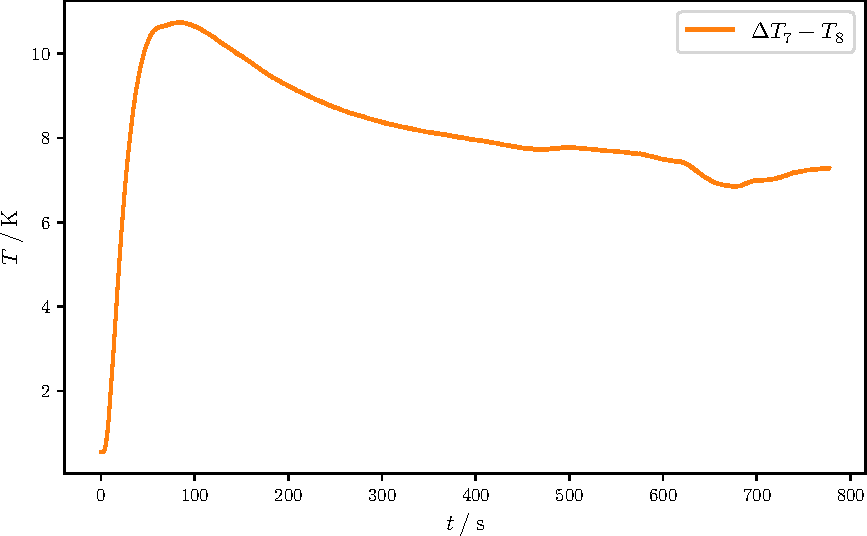
\includegraphics[width = \textwidth]{build/statDifSt.pdf}
    \caption{Temperaturdifferenz $\symup{\Delta}T_\text{St}$}
    \label{fig:statDifSt}
  \end{subfigure}
  \begin{subfigure}{0.48\textwidth}
    \centering
    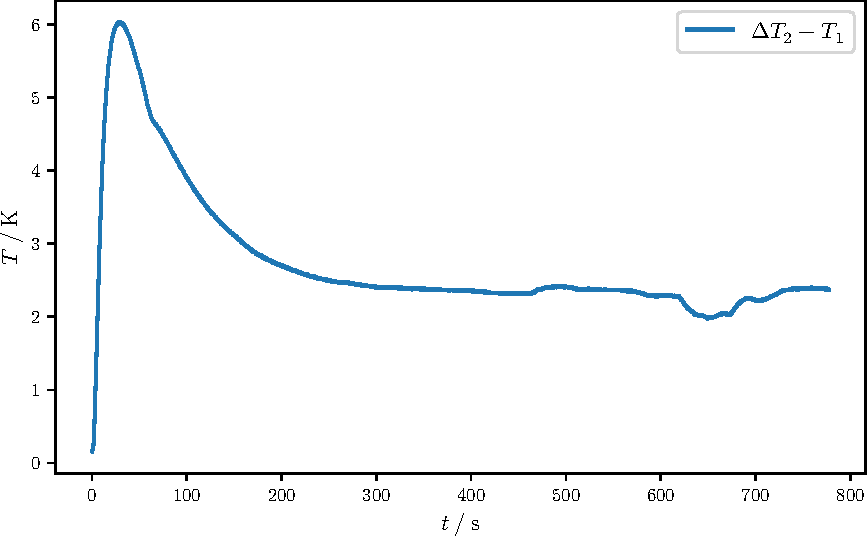
\includegraphics[width = \textwidth]{build/statDifMek.pdf}
    \caption{Temperaturdifferenz $\symup{\Delta}T_\text{Me,k}$}
    \label{fig:statDifMek}
  \end{subfigure}
\end{figure}
Bei der Betrachtung beider Grpahen erkennt man instantan, dass bei beiden Kurven ein Maximum kur vor $t = \SI{100}{\second}$ erreicht wird, wobei beide danach 
wieder abfallen. Dies lieg der Ursache zu Grunde, dass die Temperaturen an den inneren und äußeren Thermoelementen im Bereich der Raumtemperatur liegen. 
Erwärmt man jedoch den Stab steigt die Temperatur am inneren  Thermoelement deutlich schneller an als die an dem äußeren Thermoelement, da die Wärme erstmal
in einer gewissen Zeit nach außen srömen muss, so dass ein zeitlicher Verzug entsteht. Bei näherer Betrachung wird die Stärk des Abfalls auffällig, da die
Temperaturdifferenz des Stahlstabes deutlich langsamer abfällt als die des großen Messingstabes. Der Grund hierfür ist die unterschidlich hohe
Wärmeleitfähigkeit der Stäbe, welche schon durch die Tabelle \eqref{tab:Waeremleitfaehigkeit} aufgezeigt wird. Da die Wärmeleitfähigkeit des
Messingstabes besser ist, kann die Temperatur am äußeren Messpunkt schneller ansteigen, da mehr Wärme pro Zeit geleitet wird.
\subsection{Dynamisches Verfahren}
\begin{figure}
  \centering
  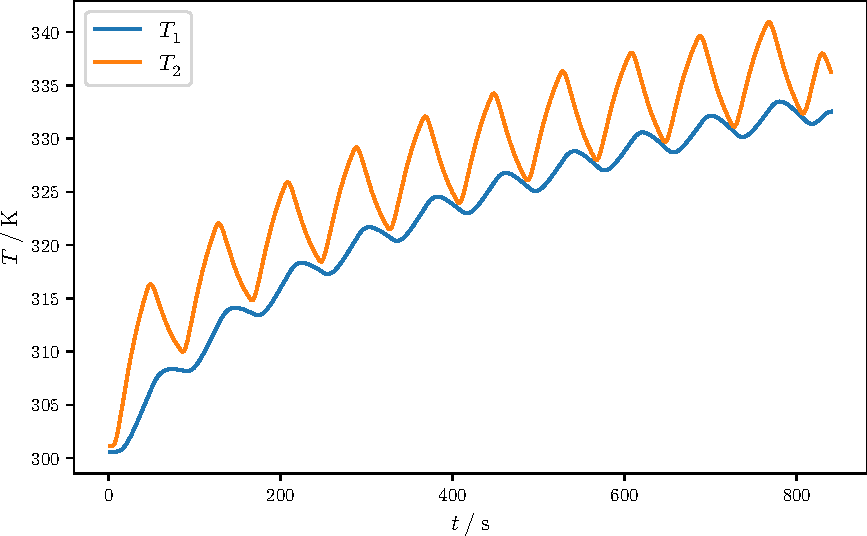
\includegraphics[width = \textwidth]{build/Me.pdf}
\end{figure}